\documentclass[11pt, addpoints, answers]{exam}

\usepackage{amsmath, amssymb}
\usepackage{xcolor}

\newcommand{\red}[1]{\textcolor{red}{#1}}

% For inserting code snippets.
\usepackage{listings}
\lstset{
    columns = fixed,
    basewidth = {0.5em},
    breaklines = true,
    backgroundcolor = \color{white},
    keywordstyle = \color[RGB]{40, 40, 255},
    numberstyle = \footnotesize\color{darkgray},
    commentstyle = \ttfamily\color{violet},
    basicstyle = \ttfamily,
    stringstyle = \ttfamily\color[RGB]{128, 0, 0},
    showstringspaces = false,
    language = {[11]C++},
    escapechar = \@
}
\lstnewenvironment{cpp}[1][]{\lstset{language = {[11]C++}, #1}}{}

\usepackage{tikz}
\usepackage{tikz-qtree}
\tikzset{every tree node/.style={minimum width=2em,draw,circle},
    blank/.style={draw=none},
    edge from parent/.style=
    {draw,edge from parent path={(\tikzparentnode) -- (\tikzchildnode)}},
    level distance=1.2cm}

% headers, footers, titles
\newcommand{\CourseName}{CS101 Algorithms and Data Structures}
\newcommand{\HomeworkNO}{Homework 6}
\newcommand{\DueDate}{Due date: November 19, 2023, at 23:59}

\pagestyle{headandfoot}
\runningheadrule
\runningheader{\CourseName}{\HomeworkNO}{\DueDate}
\runningfooter{}{\thepage}{}

\title{
	\CourseName\\
	Fall 2023\\
	\HomeworkNO
}
\author{}
\date{\DueDate}

% formats of questions, choices, points, etc.
\qformat{\bf\thequestion. (\totalpoints\ points) \thequestiontitle\hfill}
\pointname{'}
\CorrectChoiceEmphasis{\bf\color{blue}}
\SolutionEmphasis{\color{blue}}

% We frequently use this font.
\newcommand{\ttt}{\texttt}
\newcommand{\bluett}[1]{\textcolor{blue}{\ttt{#1}}}

\begin{document}

\maketitle

\begin{enumerate}
    \item Please write your solutions in English.
    \item Submit your solutions to gradescope.com.
    \item Set your FULL name to your Chinese name and your STUDENT ID correctly in Account Settings.
    \item If you want to submit a handwritten version, scan it clearly. \ttt{CamScanner} is recommended.
    \item When submitting, match your solutions to the problems correctly.
    \item No late submission will be accepted.
    \item Violations to any of the above may result in zero points.
\end{enumerate}

\begin{questions}

    \newpage

    \titledquestion{Multiple Choices}

Each question has \textbf{one or more} correct answer(s). Select all the correct answer(s). For each question, you will get 0 points if you select one or more wrong answers, but you will get 1 point if you select a non-empty subset of the correct answers.

Write your answers in the following table.

%%%%%%%%%%%%%%%%%%%%%%%%%%%%%%%%%%%%%%%%%%%%%%%%%%%%%%%%%%%%%%%%%%%%%%%%%%%
% Note: The `LaTeX' way to answer a multiple-choices question is to replace `\choice'
% with `\CorrectChoice', as what you did in the first question. However, there are still
% many students who would like to handwrite their homework. To make TA's work easier,
% you have to fill your selected choices in the table below, no matter whether you use 
% LaTeX or not.
%%%%%%%%%%%%%%%%%%%%%%%%%%%%%%%%%%%%%%%%%%%%%%%%%%%%%%%%%%%%%%%%%%%%%%%%%%%

\begin{table}[htbp]
    \centering
    \begin{tabular}{|p{2cm}|p{2cm}|p{2cm}|p{2cm}|}
        \hline
        (a) & (b) & (c) & (d) \\
        \hline
        %%%%%%%%%%%%%%%%%%%%%%%%%%%%%%%%%%%%%%%%%%%%%%%%%%%%%%%%%%
        % YOUR ANSWER HERE.
        AD  & BCD & AB  & D   \\
        %%%%%%%%%%%%%%%%%%%%%%%%%%%%%%%%%%%%%%%%%%%%%%%%%%%%%%%%%%
        \hline
    \end{tabular}
\end{table}

\begin{parts}
    \part[2] Which of the following operations on a \textbf{Linked List} take constant time?

    \begin{choices}
        \CorrectChoice Given a pointer $h$ which points to the head node of a linked list, we want to erase the head node.
        \choice Given a pointer $h$ which points to the head node of a linked list, we want to gain access to the last element of the linked list.
        \choice Given a pointer $p$ which points to a node in a linked list, we want to gain access the previous node of $p$.
        \CorrectChoice Given a pointer $p$ which points to a node in a linked list, we want to insert an element after $p$.
    \end{choices}

    \part[2] Which of the following statements about arrays and linked-lists are true?

    \begin{choices}
        \choice Inserting an element into the middle of an array takes constant time.
        \CorrectChoice A doubly linked list consumes more memory than a (singly) linked list of the same length.
        \CorrectChoice Given a pointer to some node in a doubly linked list, we are able to gain access to every node of it.
        \CorrectChoice Given a pointer to any node in a linked list, we are able to gain access to the last node.
    \end{choices}

    \part[2] Please evaluate the following reverse-Polish expressions. Which of them are legal reverse-Polish expressions and gives a result greater than 0?

    \begin{choices}
        \CorrectChoice \ttt{2 3 2 * + 1 /}
        \CorrectChoice \ttt{1 2 4 - - 3 *}
        \choice \ttt{1 * 2 - 1 + 5}
        \choice \ttt{2 4 3 1 + * -}
    \end{choices}

    \part[2] Assume we implement a queue with a circular array indexed from $0$ to $n-1$. Now the \ttt{front} pointer is at index $a$, and the \ttt{back} pointer is at index $b$. Which of the following best describes the number of the elements in the queue?

    \begin{choices}
        \choice $b-a+1$
        \choice $|b-a+1|$
        \choice $b-a+1+n$
        \CorrectChoice $(b-a+1+n) \mod n$
    \end{choices}


\end{parts}

    \newpage

    \titledquestion{AVL tree operations}

Here is an AVL tree. Denote it as $T$.
\begin{center}
    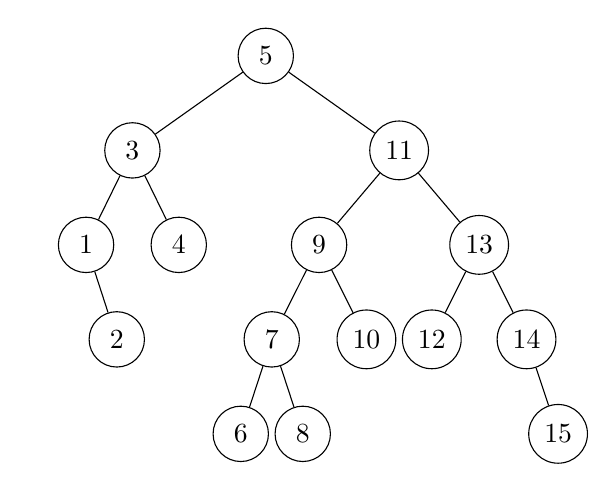
\begin{tikzpicture}[]
    \Tree
    [.5
        [.3
            [.1
                \edge[blank]; \node[blank]{};
                [.2
                ]
            ]
            [.4
            ]
        ]
        [.11
            [.9
                [.7
                    [.6
                    ]
                    [.8
                    ]
                ]
                [.10
                ]
            ]
            [.13
                [.12
                ]
                [.14
                    \edge[blank]; \node[blank]{};
                    [.15
                    ]
                ]
            ]
        ]
    ]
    \end{tikzpicture}
\end{center}

\begin{parts}

\part[2] Insert $8.5$ into $T$. Draw the AVL tree before checking if any balance correction is needed.

\vspace{7cm}

\part[2] Insert $8.5$ into $T$. Draw the AVL tree after balance corrections.

\vspace{7cm}

\part[2] Remove $3$ from $T$ (\textbf{NOT from the previous answer!}). Draw the AVL tree after replacing and before checking if any balance correction is needed.

\vspace{7cm}

\part[2] Remove $3$ from $T$. Draw the AVL tree after balance corrections.

\vspace{7cm}

\end{parts}

\end{questions}

\end{document}